\chapter{Spin Systems, Phase Transitions and Inference}
\label{ch:spins}

\section{The Ising model}

Lenz proposed in 1920~\cite{brush1967}, and his student Ising solved in 1925 in one dimension~\cite{ising1925}, a model of a magnet in which spins $\sigma_x\in\{-1,+1\}$ sit on the sites of a lattice and interact with their neighbors. On a finite graph $G = (V,E)$, with coupling $J>0$ and external field $h$, the Gibbs measure at inverse temperature $\beta$ is
\[
\mu_{\beta,h}(\sigma) = \frac{1}{Z_{\beta,h}}\exp\Big(\beta J\sum_{\{x,y\}\in E}\sigma_x\sigma_y+h\sum_{x\in V}\sigma_x\Big).
\]
Ising found no phase transition in one dimension and wrongly conjectured none in higher dimensions. Peierls showed in 1936~\cite{peierls1936} that in two dimensions there is spontaneous magnetization at low temperature, and the exact solution of Onsager and Yang is in Section~\ref{sec:onsager}.

\begin{theorem}[Peierls]
For the Ising model on $\Z^2$ with plus boundary conditions on a box $\Lambda_n$ and $h = 0$, there is $\beta_0<\infty$ such that for $\beta>\beta_0$ the probability that the spin at the origin is minus is at most $\frac13$, uniformly in $n$. Hence the infinite volume limits with plus and minus boundary conditions differ, and there is a phase transition.
\end{theorem}

\begin{proof}
Represent a configuration by its contours, the closed polygons on the dual lattice separating plus from minus spins. If the origin is minus, it is surrounded by at least one contour $\gamma$. Flipping all spins inside $\gamma$ removes it and changes the energy by $2\beta J|\gamma|$, and the map is injective for fixed $\gamma$, so $\mu(\gamma\text{ present})\leq e^{-2\beta J|\gamma|}$. The number of contours of length $\ell$ surrounding the origin is at most $\ell\,3^{\ell}$, since such a contour crosses the horizontal axis at one of at most $\ell$ points and is then a self avoiding path. Hence
\[
\mu(\sigma_0 = -1)\leq\sum_{\ell\geq4}\ell\,3^\ell e^{-2\beta J\ell},
\]
which is below $\frac13$ for $\beta$ large.
\end{proof}

The argument is an entropy against energy estimate. The same structure, a comparison of the number of bad configurations with their likelihood penalty, is the first moment method that bounds the information theoretic thresholds of inference problems below.

\section{The Lee Yang circle theorem}

Write $z = e^{-2h}$. Up to a factor $e^{h|V|}$, the partition function is a polynomial in $z$ of degree $|V|$, $Z(z) = \sum_{U\subset V}z^{|U|}\exp(\beta J\sum_{x\sim y}\sigma^U_x\sigma^U_y)$, where $U$ is the set of minus spins.

\begin{theorem}[Lee and Yang~\cite{leeyang1952}]
For ferromagnetic couplings $J_{xy}\geq0$ on any finite graph, all zeros of $Z(z)$ lie on the unit circle $|z| = 1$.
\end{theorem}

\begin{proof}[Sketch, after Asano]
Assign an independent fugacity $z_x$ to each site, so that $Z$ is multiaffine in $(z_x)$. For a single edge with $a = e^{-2\beta J}\in(0,1]$, the polynomial $P(z_1,z_2) = 1+az_1+az_2+z_1z_2$ (after normalization) does not vanish when $|z_1|<1$ and $|z_2|<1$, since $P = 0$ forces $z_2 = -(1+az_1)/(a+z_1)$, a M\"obius map sending the open unit disc to the exterior of the closed disc. The second ingredient is Asano's contraction lemma~\cite{asano1970}, which we prove below for complex numbers $A,B,C,D$. It holds also with $A,B,C,D$ polynomials in further variables ranging over a polydisc, by applying the scalar statement for each fixed value of those variables. Building the graph one edge at a time, taking products of polynomials in disjoint variables and contracting duplicated site variables, preserves nonvanishing in the open polydisc. Setting all $z_x = z$ gives $Z(z)\neq0$ for $|z|<1$, and the symmetry $Z(z) = z^{|V|}Z(1/z)$ under global spin flip gives $Z(z)\neq0$ for $|z|>1$.
\end{proof}

\begin{lemma}[Asano]
Let $P(z_1,z_2) = A+Bz_1+Cz_2+Dz_1z_2$ with $A,B,C,D\in\C$ and $P(z_1,z_2)\neq0$ whenever $|z_1|<1$ and $|z_2|<1$. Then $A+Dz\neq0$ whenever $|z|<1$.
\end{lemma}

\begin{proof}
Since $P(0,0) = A\neq0$, the claim is trivial if $D = 0$. If $D\neq0$, the polynomial $P(z,z) = A+(B+C)z+Dz^2$ has two roots whose product is $A/D$. If $|A/D|<1$, at least one root $\zeta$ satisfies $|\zeta|<1$, and then $P(\zeta,\zeta) = 0$ with $(\zeta,\zeta)$ in the open polydisc, a contradiction. Hence $|A|\geq|D|$, and $A+Dz = 0$ would force $|z| = |A/D|\geq1$.
\end{proof}

Figure~\ref{fig:lee_yang} shows the zeros for the Ising model on a $4\times4$ torus, computed by exact enumeration of the $2^{16}$ configurations. All sixteen lie on the unit circle to numerical precision, with $\big||z|-1\big|\leq1.2\times10^{-15}$. As the volume grows, the zeros accumulate on the circle with a limiting density~\cite{leeyang1952}. Above the critical temperature this density has a gap: it vanishes on an arc around $z = 1$, and the free energy is analytic at $h = 0$. The gap closes as the temperature decreases to the critical temperature, and below it the density of the zeros at $z = 1$ is proportional to the spontaneous magnetization. The zeros then touch the real axis at $z = 1$, which produces the singularity of the free energy at $h = 0$ that is the phase transition. A single small torus cannot show this limit, and its inverse temperature $\beta J = 0.6$ exceeds the critical value $\beta_cJ\approx0.4407$ of Section~\ref{sec:onsager}.

\begin{figure}[t]
\centering
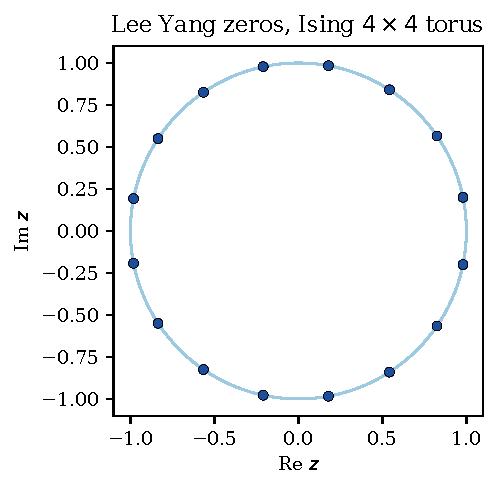
\includegraphics[width=0.62\textwidth]{lee_yang}
\caption{Lee Yang zeros of the Ising partition function on a $4\times4$ torus at $\beta J=0.6$, in the variable $z=e^{-2h}$. The largest value of $\big||z|-1\big|$ is $1.2\times10^{-15}$.}
\label{fig:lee_yang}
\end{figure}

Newman~\cite{newman1974} generalized the theorem to the ferromagnetic random variables of Chapter~\ref{ch:mixtures}, and for systems with this Lee Yang property the Griffiths, Hurst and Sherman inequality~\cite{griffiths1970}, which states that the magnetization is concave in a positive field, follows~\cite{newman1975}. In 1976 Newman~\cite{newman1976} reformulated the Riemann hypothesis in this language (Chapter~\ref{ch:open}).

\section{The Curie Weiss model and the Gaussian trick}\label{sec:curieweiss}

The mean field model has all pairs coupled with strength $1/N$:
\[
Z_N = \sum_{\sigma\in\{\pm1\}^N}\exp\Big(\frac{\beta}{2N}\Big(\sum_i\sigma_i\Big)^2+h\sum_i\sigma_i\Big).
\]
The quadratic interaction is decoupled by the Hubbard Stratonovich identity, which is the Gaussian integral $e^{a^2/2} = \E e^{aW}$ with $W\sim N(0,1)$, a scale mixture in reverse:
\[
\exp\Big(\frac{\beta}{2N}S^2\Big) = \sqrt{\frac{N\beta}{2\pi}}\int_\R\exp\Big(-\frac{N\beta m^2}{2}+\beta mS\Big)\dd m.
\]
Conditionally on $m$ the spins are independent, and summing over them gives
\begin{gather*}
Z_N = \sqrt{\frac{N\beta}{2\pi}}\int_\R\exp\big(-N\Psi(m)\big)\dd m, \\
\Psi(m) = \frac{\beta m^2}{2}-\log\big(2\cosh(\beta m+h)\big).
\end{gather*}
Laplace's method gives the free energy $-\lim N^{-1}\log Z_N = \min_m\Psi(m)$, attained where $\Psi'(m) = 0$, the mean field equation
\[
m = \tanh(\beta m+h).
\]
For $h = 0$ and $\beta\leq1$ the only solution is $m = 0$; for $\beta>1$ there are two symmetric minimizers $\pm m^*(\beta)$, and the magnetization jumps as $h$ crosses zero. The latent variable $m$ is a data augmentation: given $m$, the spins are independent with means $\tanh(\beta m+h)$, and given the spins, $m$ is Gaussian with mean $S/N$ and variance $1/(N\beta)$. The resulting two block Gibbs sampler is the Swendsen Wang idea in its simplest form, and the phase transition is visible as bimodality of the latent variable.

\section{Bayes optimal inference is a planted spin system}\label{sec:spiked}

Consider a signal $x^*\in\{\pm1\}^N$ drawn uniformly, and observations $Y_{ij} = \frac{\lambda}{N}x^*_ix^*_j+W_{ij}$ for $i<j$, with independent Gaussian noise of variance $1/N$, the spiked Wigner model. The posterior is
\[
p(x\mid Y)\propto\exp\Big(\lambda\sum_{i<j}Y_{ij}x_ix_j\Big),
\]
an Ising model with random couplings, a spin glass, whose couplings are correlated with a hidden planted configuration. Bayes optimal inference is statistical mechanics of this planted model, and the inverse temperature is fixed by the likelihood: it lies on what physicists call the Nishimori line.

\begin{theorem}[Nishimori identity]
Let $x^*\sim\pi$ take values in a standard Borel space, let $Y\mid x^*\sim p(\cdot\mid x^*)$, and, given $Y$, let $x$ and $x'$ be independent draws from the posterior $p(\cdot\mid Y)$, the conditional law of $x^*$ given $Y$, independent of $x^*$. For every bounded function $f$,
\[
\E\big[f(Y,x,x')\big] = \E\big[f(Y,x,x^*)\big].
\]
\end{theorem}

\begin{proof}
By definition of the posterior, conditionally on $Y$ the signal $x^*$ has the law $p(\cdot\mid Y)$, which is also the law of $x$ and of $x'$. Given $Y$ the three are independent. Hence $(Y,x,x^*)$ and $(Y,x,x')$ have the same law.
\end{proof}

The identity was introduced by Nishimori~\cite{nishimori1981} in 1981 for the Ising model with random bonds, using gauge transformations, and recognized in its statistical form by Iba~\cite{iba1999} and by Zdeborov\'a and Krzakala~\cite{zdeborova2016}. With a different prior or a different inverse temperature the draws are not draws from the conditional law of the signal given the data, and the identity fails in general. Taking $f(Y,x,x') = g\big(N^{-1}\langle x,x'\rangle\big)$ with $g$ bounded shows that the overlap between two posterior samples has the same law as the overlap between a posterior sample and the truth. This identity and the concentration of the overlap, which is proved separately, are the structural input of the proof of the replica symmetric formula for the mutual information by Lelarge and Miolane~\cite{lelarge2019}, who use the Aizenman Sims Starr scheme. The adaptive interpolation method of Barbier and Macris~\cite{barbier2019} gives another proof. Replica symmetry here means that the overlap has a single limiting value at equilibrium. It does not exclude metastable states, and it is compatible with the computational hardness discussed in the next section.

For the uniform sign prior of this section the replica symmetric formula for the mutual information per spin is
\[
\begin{multlined}\lim_{N\to\infty}\frac1NI(x^*;Y) = \min_{q\geq0}\Big\{\frac{\lambda^2}{4}(1-q)^2+\lambda^2q\\ -\E\log\cosh\big(\lambda^2q+\lambda\sqrt q\,\xi\big)\Big\},\end{multlined}
\]
where $\xi\sim N(0,1)$. The minimizer $q^*$ solves $q = \E\tanh(\lambda^2q+\lambda\sqrt q\,\xi)$ and is the limit of $|N^{-1}\langle x,x^*\rangle|$ for a posterior sample $x$. It vanishes for $\lambda\leq1$ and is close to $2(\lambda-1)$ just above $\lambda = 1$. The observation $\sqrt N\,Y_{ij} = \lambda\,x^*_ix^*_j/\sqrt N+\sqrt N\,W_{ij}$ is a Gaussian channel with signal to noise ratio $\lambda^2$ for the vector of products $(x^*_ix^*_j/\sqrt N)_{i<j}$, and $Y$ depends on $x^*$ only through these products. The I MMSE relation of Guo, Shamai and Verd\'u~\cite{guo2005}, Theorem~\ref{thm:immse} of Chapter~\ref{ch:entropy}, therefore gives
\begin{gather*}
\frac{\dd}{\dd(\lambda^2)}\frac1NI(x^*;Y) = \frac14\,\mathrm{mmse}_N, \\
\mathrm{mmse}_N = \frac{1}{N^2}\,\E\big\|x^*x^{*\top}-\E[x^*x^{*\top}\mid Y]\big\|_F^2.
\end{gather*}
Differentiating the replica symmetric formula gives $\mathrm{mmse}_N\to1-q^{*2}$, for all but countably many $\lambda$~\cite{lelarge2019}, so the phase transitions of the Bayes optimal error are read off from the minimizer $q^*$. For uniform signs the transition at $\lambda = 1$ is continuous. For other priors the error can jump. For sparse signals it jumps at the information theoretic threshold~\cite{lesieur2017}, and so does the optimal generalization error of the perceptron with binary weights~\cite{barbier2019b}.

\section{Statistical and computational thresholds}

The planted clique problem asks to find a clique of size $k$ planted in an Erd\H{o}s R\'enyi graph $G(n,\frac12)$. The largest clique in $G(n,\frac12)$ has size about $2\log_2n$, so a planted clique of size $k\geq(2+\varepsilon)\log_2n$ is identifiable by exhaustive search. Polynomial time algorithms are known only for $k\gtrsim\sqrt n$: spectral methods succeed for $k\geq C\sqrt n$~\cite{alon1998}, and Deshpande and Montanari~\cite{deshpande2015} showed that approximate message passing succeeds for $k\geq(1+\varepsilon)\sqrt{n/e}$, with the threshold $\sqrt{n/e}$ predicted by state evolution. Jerrum showed in 1992~\cite{jerrum1992} that from a suitable starting state the Metropolis process cannot find a planted clique of size $k = n^{1/2-\varepsilon}$ in polynomial time. The conjecture that no polynomial time algorithm succeeds for $k = n^{1/2-\varepsilon}$ is supported by lower bounds for sum of squares relaxations~\cite{barak2019} and for low degree polynomial tests~\cite{kunisky2019}, which have become a standard heuristic for computational hardness.

For Bayesian inference the lesson is that a posterior can be statistically informative and computationally inaccessible. The physical picture of the gap~\cite{zdeborova2016} is a phase transition in the landscape of the posterior: between the information theoretic and the algorithmic thresholds the posterior concentrates near the planted configuration, but a large, entropically dominant region of uninformative states separates any tractable starting point from it. A bottleneck of this kind makes the conductance of a reversible local dynamics, and with it the spectral gap and the log Sobolev constant of Chapter~\ref{ch:entropy}, exponentially small, so that Glauber or Langevin dynamics mixes slowly. This is a heuristic for hardness and not a general theorem. It has been proved for particular dynamics in particular models: the Metropolis process on the planted clique~\cite{jerrum1992}, and Langevin dynamics and gradient descent in tensor principal component analysis, where recovery from natural initializations takes at least stretched exponential time below an explicit threshold~\cite{benarous2020}. The heuristic concerns local dynamics and does not apply to spectral methods or approximate message passing. Obstructions for broader classes of algorithms come from other arguments, such as the overlap gap property~\cite{gamarnik2021}. In the physics of glasses equilibrium is likewise unattainable on accessible time scales. The analogy suggests that the gap is intrinsic, which remains a conjecture.

\section{Double descent as a phase transition}

Consider linear regression $y = X\theta+w$ with $n$ observations, $p$ isotropic Gaussian features, $\|\theta\|^2 = r^2$ and noise variance $\sigma^2$, in the proportional limit $p/n\to\psi$. Ridge regression with penalty $\alpha>0$ minimizes $n^{-1}\|y-X\theta\|^2+\alpha\|\theta\|^2$. The minimum norm least squares estimator, the limit of ridge regression as the penalty vanishes, has asymptotic prediction risk, by Hastie, Montanari, Rosset and Tibshirani~\cite{hmrt2022},
\[
R(\psi) = \begin{cases}\sigma^2\dfrac{\psi}{1-\psi}, & \psi<1,\\[2ex] r^2\Big(1-\dfrac1\psi\Big)+\dfrac{\sigma^2}{\psi-1}, & \psi>1.\end{cases}
\]
The risk diverges at the interpolation threshold $\psi = 1$ and then descends again, the double descent phenomenon. The divergence is a phase transition in the sense of this chapter: the smallest singular value of $X$ vanishes at $\psi = 1$, the Marchenko Pastur law reaching zero, and the inverse that defines the estimator blows up.

The Bayes posterior mean under the Gaussian prior with the correct signal and noise levels is ridge regression with penalty $\alpha = \sigma^2\psi/r^2$, and its risk is monotone in $\psi$ with no peak. Suppose instead that the penalty is held fixed while the number of features grows. The penalty corresponds to the working Gaussian prior $N(0,(\sigma^2/(n\alpha))I)$, which then no longer matches the signal. In our paper on Bayesian double descent~\cite{polsonsokolov2025dd} we show, for $\rho = r^2/\sigma^2$, that the limiting risk of ridge regression with fixed penalty $\alpha$ is nondecreasing in $\psi$ if and only if $\alpha\geq\alpha_c(\rho)$. The critical penalty $\alpha_c(\rho)$ is finite if and only if $\rho\geq1$, and $\alpha_c(2) = 1/11$. For $\alpha<\alpha_c(\rho)$ the risk has an interior maximum followed by a decreasing stretch, which is the double descent. Having more parameters than observations does not by itself produce the peak. It appears when the working prior is more diffuse than a critical level.

\section{Samplers from physics}

The Metropolis algorithm was invented at Los Alamos in 1953~\cite{metropolis1953} to compute the equation of state of a system of hard discs, the same system whose kinetic limit Lanford studied twenty years later. Glauber dynamics, heat bath updates of single spins, is the Gibbs sampler of statistics. Both suffer from critical slowing down near phase transitions, where the spectral gap closes.

Swendsen and Wang introduced in 1987~\cite{swendsen1987} a cluster algorithm that flips large clusters of aligned spins at once. Edwards and Sokal~\cite{edwards1988} explained it as data augmentation: introduce bond variables $\omega_{xy}\in\{0,1\}$ with joint law proportional to
\begin{gather*}
\prod_{\{x,y\}\in E}\Big((1-p)\mathbb{1}\{\omega_{xy} = 0\}+p\,\mathbb{1}\{\omega_{xy} = 1\}\mathbb{1}\{\sigma_x = \sigma_y\}\Big), \\
p = 1-e^{-2\beta J},
\end{gather*}
whose spin marginal is the Ising measure and whose bond marginal is the Fortuin Kasteleyn random cluster model. Given the spins, bonds are independent; given the bonds, clusters are assigned independent uniform spins. The algorithm is a two block Gibbs sampler on the augmented space, and it mixes rapidly at temperatures where single spin dynamics does not.

The slice sampler is the same idea in statistics: to sample a density $\pi(x)$, introduce $u\mid x\sim U(0,\pi(x))$ and sample $x\mid u$ uniformly on $\{\pi\geq u\}$. Damien, Wakefield and Walker~\cite{damien1999} developed it for Bayesian models, and Neal~\cite{neal2003} gave a general treatment. Augmentation can also fail. The witch's hat example of Polson in the discussion of Geyer's paper on practical Markov chain Monte Carlo~\cite{polson1992} exhibits a density, a narrow spike on a broad base, for which the Gibbs sampler and other local samplers appear to converge while missing a region of substantial mass; it is a phase coexistence problem in miniature, and it shows why diagnostics based on a single run cannot certify convergence. Rigorous complexity bounds for sampling log concave densities begin with the random walk algorithm of Dyer, Frieze and Kannan~\cite{dyer1991} for the uniform density on a convex body, which Applegate, Kannan and Polson~\cite{akp1990}, Applegate and Kannan~\cite{applegate1991} and Frieze, Kannan and Polson~\cite{frieze1994} extended to log concave densities. The analysis bounds the conductance of the walk, and through it the spectral gap, by isoperimetric inequalities of the kind proved for convex bodies by Lov\'asz and Simonovits~\cite{lovasz1993} and by Kannan, Lov\'asz and Simonovits~\cite{kannan1995}. These inequalities are quoted here without proof. Chapter~\ref{ch:poincare} relates the spectral gap to the Poincar\'e inequality and proves the inequality for the Gaussian measure, Theorem~\ref{thm:gaussian_poincare}.

\section{Onsager's solution and the critical point}\label{sec:onsager}

Onsager's 1944 solution~\cite{onsager1944} of the two dimensional Ising model on the square lattice with coupling $J$ and zero field gives the free energy per site
\[
\begin{multlined}-\beta f = \log2+\frac{1}{2\pi^2}\int_0^\pi\!\!\int_0^\pi\log\Big(\cosh^2(2\beta J)\\ -\sinh(2\beta J)\big(\cos k_1+\cos k_2\big)\Big)\dd k_1\dd k_2.\end{multlined}
\]
The integrand vanishes at $k_1 = k_2 = 0$ exactly when $\cosh^2(2\beta J) = 2\sinh(2\beta J)$, that is $\sinh(2\beta_cJ) = 1$, so the critical point is $\beta_cJ = \frac12\log(1+\sqrt2)\approx0.4407$, the value predicted earlier by Kramers and Wannier~\cite{kramers1941} from the duality between high and low temperature expansions. The specific heat diverges logarithmically at $\beta_c$. The spontaneous magnetization, announced by Onsager and proved by Yang in 1952~\cite{yang1952}, is
\[
m^*(\beta) = \big(1-\sinh^{-4}(2\beta J)\big)^{1/8},\qquad\beta>\beta_c,
\]
vanishing at $\beta_c$ with exponent $\frac18$. Mean field theory predicts the exponent $\frac12$, so the two dimensional model is a rigorous counterexample to the universality of mean field exponents. The exact solution showed for the first time that a phase transition with nonclassical exponents can follow from a microscopic model by pure mathematics, a demonstration of the derivational reading of the sixth problem in equilibrium statistical mechanics.

\section{The Gibbs variational principle and variational inference}

\begin{theorem}[Gibbs variational principle]
Let $\nu$ be a probability measure on a space $\Omega$ and $H:\Omega\to\R$ measurable with $Z = \int e^{H}\dd\nu<\infty$. Then
\[
\log Z = \sup_Q\Big\{\int H\dd Q-\KL(Q\,\|\,\nu)\Big\},
\]
the supremum over probability measures $Q$ with $\int|H|\dd Q<\infty$. If in addition $\int|H|e^{H}\dd\nu<\infty$, which is equivalent to $\KL(Q^*\,\|\,\nu)<\infty$, the supremum is attained, uniquely at $Q^*(\dd\omega) = Z^{-1}e^{H(\omega)}\nu(\dd\omega)$.
\end{theorem}

\begin{proof}
Let $Q$ be a probability measure with $\int|H|\dd Q<\infty$. If $Q$ is not absolutely continuous with respect to $\nu$, then $\KL(Q\|\nu) = \infty$ and the functional being maximized is $-\infty$. Otherwise $Q\ll Q^*$ and $\frac{\dd Q}{\dd Q^*} = Ze^{-H}\frac{\dd Q}{\dd\nu}$, so that $\KL(Q\|Q^*) = \KL(Q\|\nu)-\int H\dd Q+\log Z$. Hence $\int H\dd Q-\KL(Q\|\nu) = \log Z-\KL(Q\|Q^*)\leq\log Z$, with equality if and only if $Q = Q^*$. This gives the upper bound, the uniqueness, and the attainment whenever $Q^*$ is admissible, that is, whenever $\int|H|\dd Q^* = Z^{-1}\int|H|e^H\dd\nu<\infty$. In general let $Q_n$ be $Q^*$ conditioned on $\{|H|\leq n\}$. It is admissible, and the same computation gives $\int H\dd Q_n-\KL(Q_n\|\nu) = \log Z+\log Q^*(|H|\leq n)$, which tends to $\log Z$.
\end{proof}

The theorem is the Gibbs variational principle of statistical mechanics, in the form of the variational formula for relative entropy of Donsker and Varadhan~\cite{donsker1975}. With $\nu$ the prior, $H$ the log likelihood and $Q^*$ the posterior, it says that Bayes' rule is the solution of a variational problem and that the log marginal likelihood is a free energy. Restricting $Q$ to a tractable family gives a lower bound, the evidence lower bound of variational inference, whose gap is the Kullback Leibler divergence from the family to the posterior. Restricting to product measures gives mean field theory.

For the Curie Weiss model of Section~\ref{sec:curieweiss}, take $\nu$ uniform on $\{\pm1\}^N$ and $H_N(\sigma) = \frac{\beta}{2N}\big(\sum_i\sigma_i\big)^2+h\sum_i\sigma_i$, so that $Z_N = 2^N\int e^{H_N}\dd\nu$. The product measure $Q_m$ with mean $m$ at every site has $\KL(Q_m\|\nu) = N\big(\log2-s(m)\big)$, where $s(m) = -\frac{1+m}{2}\log\frac{1+m}{2}-\frac{1-m}{2}\log\frac{1-m}{2}$ is the binary entropy, and $\int H_N\dd Q_m = N\big(\frac{\beta m^2}{2}+hm\big)+\frac\beta2(1-m^2)$. The theorem therefore gives $N^{-1}\log Z_N\geq\varphi(m)$ for every $m\in[-1,1]$, where $\varphi(m) = \frac{\beta m^2}{2}+hm+s(m)$. This is not the function $-\Psi(m)$ of the Hubbard Stratonovich computation. Since $\log(2\cosh u) = \max_{m'}\{um'+s(m')\}$, attained at $m' = \tanh u$, we have $-\Psi(m) = \max_{m'}\{(\beta m+h)m'+s(m')\}-\frac{\beta m^2}{2}$. Taking $m' = m$ gives $-\Psi(m)\geq\varphi(m)$, with equality if and only if $m = \tanh(\beta m+h)$. Maximizing over $m$ first, which gives $\frac{\beta m'^2}{2}$, shows that $\max_m(-\Psi) = \max_{m'}\varphi$. The two functions thus have the same stationary points, the solutions of the mean field equation, and the same maximum, which is the limit of $N^{-1}\log Z_N$. For the Curie Weiss model the product bound is therefore sharp. Mean field theory in physics and variational Bayes in statistics are the same approximation, with the same failure mode: a product family cannot represent the correlations that dominate near a phase transition.

\section{Belief propagation and the Bethe approximation}

On a tree, marginals of a Gibbs measure can be computed exactly by passing messages along edges: the message from $x$ to $y$ summarizes the effect of the subtree behind $x$, and marginals are products of incoming messages. For the Ising model with fields $h_x$ and couplings $J_{xy}$, writing messages as effective fields $u_{x\to y}$, the update is
\[
u_{x\to y} = \operatorname{artanh}\Big(\tanh(\beta J_{xy})\tanh\Big(h_x+\sum_{z\sim x,z\neq y}u_{z\to x}\Big)\Big).
\]
On graphs with cycles the same iteration, loopy belief propagation, computes stationary points of the Bethe free energy~\cite{yedidia2005}, a variational approximation that is exact on trees and accurate on locally tree like graphs. Pearl introduced belief propagation for Bayesian networks in 1982~\cite{pearl1982}, Gallager had used it for decoding in 1963~\cite{gallager1963}, and the cavity method of M\'ezard, Parisi and Virasoro is its replica symmetric physics~\cite{mezard2009}. Approximate message passing~\cite{donoho2009,bayati2011}, used earlier in this chapter for the planted clique, is its dense graph limit, and its state evolution, a one dimensional recursion for the effective signal to noise ratio, is the mechanism by which algorithmic thresholds such as $\sqrt{n/e}$ are computed.

\section*{Exercises}
\begin{enumerate}
\item Solve the one dimensional Ising model on a ring by the transfer matrix method and show that there is no phase transition at positive temperature.
\item Verify directly that the zeros of the partition function of a single Ising bond in a uniform field lie on the unit circle.
\item Show that the Curie Weiss mean field equation with $h = 0$ and $\beta>1$ has three solutions, and determine which minimize $\Psi$.
\item Prove that the Edwards Sokal measure has the Ising measure as its spin marginal.
\item Show that ridge regression with penalty $\alpha$, the minimizer of $n^{-1}\|y-X\theta\|^2+\alpha\|\theta\|^2$, is the posterior mean under the prior $N(0,(\sigma^2/(n\alpha))I)$ and Gaussian noise of variance $\sigma^2$.
\end{enumerate}


\section*{Notes}

Friedli and Velenik~\cite{friedli2017} give a modern mathematical treatment of the Ising model, including the Peierls argument, correlation inequalities and the Lee Yang theorem. Zdeborov\'a and Krzakala~\cite{zdeborova2016} survey the statistical physics of inference. M\'ezard and Montanari's \emph{Information, Physics, and Computation}~\cite{mezard2009} develops message passing and the cavity method. Barbier and Macris~\cite{barbier2019c} give an introduction to the adaptive interpolation method for the Curie Weiss and Wigner spike models.
